\documentclass[Afour,sageh,times]{sagej}

\usepackage{amsmath,amssymb,amsthm}
\usepackage{booktabs}
\usepackage{graphicx}
\usepackage{url}
\usepackage[colorlinks,citecolor=black,linkcolor=black,urlcolor=black]{hyperref}

\newtheorem{proposition}{Proposition}
\newtheorem{corollary}{Corollary}
\newcommand{\E}{\mathbb{E}}
\newcommand{\Prob}{\mathbb{P}}
\setcounter{secnumdepth}{3}
\AtBeginDocument{\onecolumn}

% plain front matter and running heads (the template placeholders are not used)
\makeatletter
\def\@maketitle{\null
  \begin{center}{\sffamily\Large\bfseries\@title\par}\vskip 1.2em
  {\sffamily\@author\par}\end{center}\vskip 1.5em
  {\noindent\usebox\absbox\par}\vskip 1em {\noindent\normalsize\@keywords\par}\vskip 1.5em}
\def\ps@title{\def\@oddhead{}\def\@evenhead{}\def\@oddfoot{\hfill\thepage\hfill}\let\@evenfoot\@oddfoot}
\def\ps@sagepage{\def\@evenhead{\small\sagesf\thepage\hfill\leftmark}\def\@oddhead{\small\sagesf\leftmark\hfill\thepage}%
  \def\@evenfoot{}\def\@oddfoot{}}
\makeatother
\AtBeginDocument{\pagestyle{sagepage}}

\begin{document}

\runninghead{Anytime-valid monitoring of survey series}

\title{Anytime-valid monitoring of repeated survey estimates under questionnaire redesign: An application to the Business Trends and Outlook Survey}

\author{Author information removed for anonymous peer review}

\begin{abstract}
Statistical agencies release survey estimates every few weeks, and users read each release as it arrives, asking whether growth has changed course. Repeated significance testing on such a stream does not control error rates, and questionnaire redesigns create discontinuities that are easily mistaken for real change. We propose a monitor for the curvature of a published series. The null hypothesis is that the latent path is locally linear with unknown level and slope, with a separate unknown level for each questionnaire regime. A mixture e-process for the quadratic term, built on the residuals after removing these nuisance parameters, is valid under continuous inspection and optional stopping. We remove the main assumptions behind the basic version in turn: a scale-invariant version is valid when the published standard errors are wrong by an unknown common factor, regime-specific slopes cover proportional redesign effects, guard waves cover regime dates that are off by one wave, and a mixture over the prior scale removes the tuning constant. Simulations with the sampling errors of the survey show where each version holds its level and what it costs in power. Applied to 56 waves of the U.S. Census Bureau's Business Trends and Outlook Survey on artificial intelligence use, the monitors agree on an acceleration in spring 2025 and on a deceleration in early 2024 that is triggered by a single large drop; they disagree on the summer 2025 slowdown, which depends on how accurate the published standard errors are.
\end{abstract}

\keywords{sequential monitoring, e-values, survey redesign, repeated surveys, official statistics}

\maketitle

\section{Introduction}
\label{sec:intro}

National statistical offices increasingly publish short-period estimates from rolling surveys. The U.S. Census Bureau's Business Trends and Outlook Survey (BTOS) releases national, sector, state and size-class estimates every two weeks \citep{censusmethod2025}. Users, from journalists to central bank staff, read each release against its predecessors and ask whether the path of an indicator has changed, for example whether the adoption of a new technology has accelerated or stalled \citep{bonney2024,fed2026,mcelheran2024}. Two features of this practice are not handled by standard inferential tools.

The first is continuous inspection. A user who applies a conventional test at every release, and who may stop at any time, faces an error rate that is not the nominal one \citep{armitage1969}. The second is redesign. Agencies revise questions, weighting and frames, and the published series then contains a discontinuity that is not a feature of the population. The survey literature handles this with models for repeated surveys that include an intervention or a parallel run, estimated by state-space methods that can be run in real time \citep{scott1974,vandenbrakel2010,ohara2019,durbin2012}. These methods estimate the size of the discontinuity and of the underlying slope, which is what an analyst usually wants, but they do not give finite-sample error control for a user who inspects the series after every release.

Sequential analysis \citep{wald1945,page1954,brown1975,lan1983,chu1996} and its modern form based on e-values and test martingales \citep{howard2021,vovk2021,ramdas2023,grunwald2024,shin2023}, including always-valid monitoring of online experiments \citep{johari2022}, provide tests with error control that is uniform over time. We combine this with the removal of nuisance parameters by projection onto the residual space, in the spirit of invariance arguments for e-values \citep{perezortiz2024}. The construction is a Robbins mixture martingale for one coefficient of a Gaussian regression with known variances; its novelty lies in the choice of the null (local linearity with a separate level for each questionnaire regime), in the treatment of regimes that enter the design sequentially, and in the evaluation on a real survey series, not in the martingale itself.

The contributions are as follows. First, a monitor for curvature of a published survey series with a closed form and a proof of validity for all values of the level, the slope and the regime offsets (Section \ref{sec:method}). Second, extensions that remove the assumptions on which the basic monitor fails: unknown scale of the published standard errors, proportional redesign effects, regime dates that are off by one wave, and the choice of prior scale (Subsection \ref{sec:extensions}). Third, a simulation study that reports where each version holds its level, what it costs in power, and where it still fails (Section \ref{sec:simulation}). Fourth, an application to 56 BTOS waves in which we report how each declaration changes across the versions, and compare the monitor with a local-linear-trend state-space model that estimates the slope directly (Section \ref{sec:application}).

\section{Setting}
\label{sec:setting}

Let $j = 1, 2, \dots$ index published waves, with release times $t_j$ measured in two-week units and published estimates $y_j$ with design-based standard errors $s_j$. Each wave carries a questionnaire regime label $r_j \in \{1, \dots, K\}$ that is fixed by the agency before the estimate is released. We write $w_j = 1/s_j^2$. The model for the published estimate is
\begin{equation}
y_j = \theta(t_j) + \mu_{r_j} + \varepsilon_j, \qquad \varepsilon_j \sim \mathcal{N}(0, s_j^2) \text{ independently},
\label{eq:model}
\end{equation}
where $\theta$ is a smooth latent path and $\mu_r$ is the offset of regime $r$ relative to the first regime. A redesign changes $\mu_r$ and leaves $\theta$ unchanged. The model is additive on the scale of the estimate: a redesign that rescales the series, or that changes its dynamics, is outside it. The standard errors $s_j$ are treated as known and as fixed in advance, as is customary in the analysis of published time series; Subsections \ref{sec:typeI} and \ref{sec:dispersion} examine what happens when they are too small. The normal approximation is reasonable at the sample sizes involved, and consecutive waves are drawn from different rotation panels \citep{censusmethod2025}, although a panel returns after twelve weeks and rotation group effects are a known source of bias in panel surveys \citep{bailar1975}.

The question asked of the series is about shape: over a stretch of consecutive waves, is the growth rate constant, or has it changed? For an epoch beginning at wave $j_0$ the null hypothesis is
\begin{equation}
H_0:\quad \theta(t) = a + b\,t \quad \text{for some } a, b \in \mathbb{R},
\label{eq:null}
\end{equation}
with $a$, $b$ and the regime offsets $\mu_r$ unknown. The alternative is constant curvature, $\theta(t) = a + b\,t + \gamma t^2/2$, with $\gamma > 0$ for acceleration and $\gamma < 0$ for deceleration. A sustained change of the growth rate in one direction has a nonzero projection on the quadratic term and is detected as a departure from $H_0$. Exact linearity is a null that no smooth path satisfies, so Subsection \ref{sec:eprocess} also gives a version with a tolerance for small curvature.

\section{Method}
\label{sec:method}

\subsection{A mixture e-process for curvature}
\label{sec:eprocess}

Fix an epoch and consider its first $n$ waves. Let $D_n$ be the $n \times p$ matrix whose columns are the indicators of the regimes present and the time variable $t_j$, let $W_n = \mathrm{diag}(w_1, \dots, w_n)$, and let $q_j = t_j^2/2$. Define $M_n = I - D_n (D_n^\top W_n D_n)^{-1} D_n^\top W_n$ and
\begin{equation}
A_n = q^\top W_n M_n\, y, \qquad B_n = q^\top W_n M_n\, q,
\label{eq:AB}
\end{equation}
with $q$ and $y$ truncated to the first $n$ waves. Here $B_n$ is the information about $\gamma$ after the level of each regime and the common slope have been removed by weighted least squares, and $A_n/B_n$ is the corresponding estimate of $\gamma$, with standard error $B_n^{-1/2}$. Neither depends on how $t_j$ is centred.

For a prior scale $\tau > 0$ on $\gamma$ (in percentage points per squared wave) and a tolerance $\gamma_0 \ge 0$, the one-sided half-normal mixtures are
\begin{equation}
E_n^{+} = \frac{2}{\tau\sqrt{a_n}}\, \Phi\!\left(\frac{A_n^{+}}{\sqrt{a_n}}\right) \exp\!\left(\frac{(A_n^{+})^2}{2 a_n}\right), \qquad
E_n^{-} = \frac{2}{\tau\sqrt{a_n}}\, \Phi\!\left(\frac{A_n^{-}}{\sqrt{a_n}}\right) \exp\!\left(\frac{(A_n^{-})^2}{2 a_n}\right),
\label{eq:E}
\end{equation}
where $a_n = B_n + \tau^{-2}$, $A_n^{+} = A_n - \gamma_0 B_n$, $A_n^{-} = -A_n - \gamma_0 B_n$ and $\Phi$ is the standard normal distribution function. With $\gamma_0 = 0$ this is the closed form of $\int_0^\infty \exp(\gamma A_n - \gamma^2 B_n/2)\,\pi_\tau(d\gamma)$, with $\pi_\tau$ the half-normal law \citep{robbins1970}; for $\gamma_0 > 0$ the likelihood ratio is taken against the boundary value $\gamma_0$, and the formula is the same with $A_n$ shifted by $\gamma_0 B_n$. The statistic $E_n^{+}$ is evidence for acceleration and $E_n^{-}$ for deceleration. Monitoring starts at the first wave $n$ with $B_n > 0$, which is the third wave of an epoch whose waves share a regime.

\begin{proposition}
\label{prop:valid}
Let $\alpha \in (0,1)$. Suppose model \eqref{eq:model} holds with $t_j$, $s_j$ and $r_j$ known in advance, and $\gamma \le \gamma_0$ (that is, $H_0$ when $\gamma_0 = 0$). Then for every $a$, $b$ and regime offsets $\mu_r$,
\[
\Prob\big(\exists\, n:\ E_n^{+} \ge 2/\alpha\big) \le \alpha/2,
\]
and likewise for $E^{-}$ when $\gamma \ge -\gamma_0$. The probability that either monitor ever reaches $2/\alpha$ is therefore at most $\alpha$.
\end{proposition}

The proof is in Appendix \ref{app:proof}. The guarantee holds at all times simultaneously, so the user may inspect the series after every release and stop at any time. The declaration rule is the first time either monitor reaches $2/\alpha$ ($40$ for $\alpha = 0.05$). Below the threshold the e-values are not given verbal labels, because under the null the probability that $E^{+}$ or $E^{-}$ ever exceeds a moderate level is not small: over 52 looks it is about $0.58$ for a level of 2 and $0.09$ for 10. As a summary of the evidence in an epoch without a declaration we report the anytime-valid p-value $\min\{1, 2/\max_n \max(E_n^{+}, E_n^{-})\}$.

\subsection{Redesigns as nuisance levels}
\label{sec:redesign}

The regime offsets $\mu_r$ enter $D_n$ as separate columns. A new regime adds a column that is zero on all earlier rows, so the residual $\sigma$-fields used in the proof remain nested. Proposition \ref{prop:valid} then holds for every value of the offsets, and a redesign that shifts the level by a constant of any size cannot produce a false declaration. Three conditions are needed and none is innocuous. The shift must be additive on the scale of the series; the post-redesign slope and curvature must be the same as before the redesign; and the regime label must be placed at the correct wave. Subsection \ref{sec:redesignsim} shows that a proportional effect, or a label that is off by one wave, destroys the guarantee of the basic monitor; Subsection \ref{sec:extensions} gives versions that do not need these conditions. The size of the jump is not used, which costs information: a regime with one wave is absorbed completely, and a regime with two waves contributes one within-regime difference, so over a short post-redesign run the regime-aware monitor is equivalent to dropping the transition wave.

For comparison we also report the pooled analysis, in which the regime columns are dropped and the spliced series is treated as one regime.

\subsection{Epochs and restarts}
\label{sec:epochs}

After a declaration the monitor starts a new epoch at the following wave, with fresh level and slope parameters.

\begin{corollary}
\label{cor:epochs}
Suppose the latent path is linear on the epoch's span so far. For an epoch beginning at a stopping time, the conditional probability that it ends in a declaration is at most $\alpha$. If the latent path is linear throughout, the number $N$ of declarations satisfies $\Prob(N \ge m) \le \alpha^m$ and $\E[N] \le \alpha/(1-\alpha)$.
\end{corollary}

This is the sense of error control for a sequence of declarations. It says that a declaration is rarely spurious when the path is linear. It says nothing when the path is not linear, which for any smooth adoption curve is the typical case: a declaration then records that the epoch's path has curved, and with the information $B_n$ growing, small curvature is eventually declared. The tolerance $\gamma_0$ addresses this: with $\gamma_0 > 0$ the guarantee holds for every path whose curvature stays below $\gamma_0$. A declaration is also a crossing time, not an estimate of when the change occurred, and the dates depend on where the epoch starts. We therefore report the estimated curvature $A_n/B_n$ with its standard error at each declaration.

\subsection{Cross-strata attribution check}
\label{sec:diagnostic}

When an agency announces a redesign the regime label is known. When it does not, the label may have to be inferred. Let $z_{k,j}$ be the standardized change in stratum $k$ between waves $j-1$ and $j$. An instrument event moves every stratum in the same wave, with the same sign and with magnitudes far above the stratum's own distribution of within-regime movements, whereas a change in the latent path builds up over several waves. We compare the change of each stratum with the 95th percentile of its own within-regime $|z_{k,j}|$, and count the strata beyond it with the same sign. This is a screening rule with no formal error control. We apply it to every wave and not only to announced redesigns.

\subsection{Constants}
\label{sec:constants}

The level is $\alpha = 0.05$, and each monitor is run at threshold $2/\alpha = 40$. The prior scale $\tau = 0.01$ percentage points per squared wave is a change of 0.1 points per wave in the growth rate accumulating over ten waves. This scale is not derived from a power calculation; the value was used in all analyses reported here, but other values were not excluded in advance, and the results for $\tau$ between 0.0025 and 0.04 are reported in Subsection \ref{sec:sensitivity}. Validity does not depend on $\tau$, only power and delay do, and Subsection \ref{sec:extensions} gives a mixture over a grid of prior scales that removes the choice. The tolerance is $\gamma_0 = 0$ unless stated.

\subsection{Extensions}
\label{sec:extensions}

Unknown scale of the standard errors. Suppose that the published standard errors are correct up to an unknown common factor, $\varepsilon_j \sim \mathcal{N}(0, \kappa^2 s_j^2)$ with $\kappa > 0$ unknown. The nuisance parameters are now the level, the slope, the regime offsets and $\kappa$. Let $\nu_n = n - \mathrm{rank}(D_n)$ be the residual degrees of freedom, $\mathrm{RSS}_n = y^\top W_n M_n y$, $s_n = A_n/\sqrt{\mathrm{RSS}_n}$ and $J(a,\nu) = \int_0^\infty r^{\nu-1} e^{-r^2/2 + a r}\, dr$. For a standardized curvature $\delta = \gamma/\kappa > 0$ define
\begin{equation}
L_n(\delta) = e^{-\delta^2 B_n/2}\, \frac{J(\delta s_n, \nu_n)}{J(0, \nu_n)}, \qquad E_n^{\sigma,+} = \int_0^\infty L_n(\delta)\, \pi_\tau(d\delta),
\label{eq:unknown}
\end{equation}
with $\pi_\tau$ the half-normal law, and $E_n^{\sigma,-}$ with $s_n$ replaced by $-s_n$. Monitoring starts when $\nu_n \ge 2$. The integral over $\delta$ has no closed form and is computed numerically on a grid concentrated at the prior quantiles and at the maximum of the integrand.

\begin{proposition}
\label{prop:scale}
Suppose model \eqref{eq:model} holds with $\varepsilon_j \sim \mathcal{N}(0, \kappa^2 s_j^2)$ and $\gamma = 0$. Then for every $a$, $b$, $\mu_r$ and $\kappa > 0$, $(E_n^{\sigma,\pm})$ is a nonnegative martingale with mean one, and $\Prob(\exists\, n:\ E_n^{\sigma,\pm} \ge 2/\alpha) \le \alpha/2$.
\end{proposition}

The proof is in Appendix \ref{app:proof}. The price of the unknown scale is a loss of the information on the size of the errors in the first waves of each epoch and a numerical integral. The proposition covers the point null $\gamma = 0$; a tolerance is not combined with it here.

Proportional redesign effects and misdated regimes. If the post-redesign path is a multiple of the pre-redesign path, then within each regime the path is still linear, with a different slope. The nuisance space can therefore contain a separate slope for each regime, and the monitor then tests only for curvature within regimes. Proposition \ref{prop:valid} applies unchanged, because the added columns only enlarge $D_n$. If the regime date is known to within $g$ waves, the $2g+1$ waves around the announced date can be given a level of their own and are absorbed. We call this the guard. Regime slopes and guard waves can be combined; both cost information, which Table \ref{tab:variants} quantifies.

Scale of the series. If the redesign effect is multiplicative, a log transformation with delta-method standard errors $s_j/y_j$ makes it additive; the null is then that the log series is linear, that is, exponential growth at a constant rate. The choice of scale is a substantive choice: it determines what is called curvature.

Mixture over the prior scale. A convex combination of e-processes is an e-process. We use the equal-weight mixture of $E^{\pm}_n$ over $\tau \in \{0.0025, 0.005, 0.01, 0.02, 0.04\}$, which is valid under the same conditions as the single-scale processes and removes the choice of $\tau$.

\section{Simulation study}
\label{sec:simulation}

All simulations use the dates and design-based standard errors of the 54 legacy-wording BTOS waves, with 20,000 replications unless stated. Five rules monitor the curvature statistic $A_n/\sqrt{B_n}$ over the 52 looks from the third wave. The e-process uses $\tau = 0.01$ and $\alpha = 0.05$. The Bonferroni rule uses level $\alpha/52$ at each look and needs the horizon in advance. The spending rule uses level $\alpha/(k(k+1))$ at look $k$ and does not. The exact boundary is a constant threshold on $|A_n|/\sqrt{B_n}$, calibrated by simulation to size 0.05 for this design; it needs the horizon and the information schedule. The uncorrected rule tests at level $\alpha$ at every look. The simulation code is part of the replication package.

\subsection{False-declaration probability}
\label{sec:typeI}

\begin{table}[t]
\small\centering
\caption{Probability of at least one declaration over 52 looks (20,000 replications; nominal level 0.05). The first three rows are valid cases; correlated errors use a lag-6 autoregressive structure at the stated correlation, and standard errors are too small by the stated factor. Rows 4 to 10 use slope 0.15.}
\label{tab:typeI}
\begin{tabular}{lcccc}
\toprule
Scenario & E-process & Bonferroni & Spending & Uncorrected \\
\midrule
Linear null, slope 0.00 & 0.020 & 0.024 & 0.044 & 0.600 \\
Linear null, slope 0.15 & 0.019 & 0.023 & 0.042 & 0.601 \\
Linear null, slope 0.30 & 0.018 & 0.025 & 0.046 & 0.602 \\
Overlap correlation 0.25 & 0.011 & 0.022 & 0.043 & 0.573 \\
Overlap correlation 0.50 & 0.006 & 0.019 & 0.043 & 0.498 \\
Standard errors understated by 10\% & 0.048 & 0.062 & 0.084 & 0.738 \\
Standard errors understated by 25\% & 0.120 & 0.168 & 0.180 & 0.875 \\
Standard errors understated by 50\% & 0.314 & 0.415 & 0.397 & 0.973 \\
\bottomrule
\end{tabular}

\end{table}

Table \ref{tab:typeI} shows that the e-process holds its level for all three slopes at about 0.02, below the nominal 0.05, because the mixture and the two-sided split are conservative at this horizon. The Bonferroni rule is similar at 0.023 to 0.025, the spending rule uses most of the budget (0.043 to 0.046), the exact boundary reaches its size of 0.05 by construction, and the uncorrected rule declares at least once in 60 percent of replications, 2.6 times on average. Over the full restart procedure under a linear path the probability of at least one declaration is 0.022 and the expected number of declarations is 0.022 (slope 0) and 0.024 (slope 0.3), within the bound of Corollary \ref{cor:epochs}. Lag-6 correlation, as when a rotating panel returns, makes the e-process, the Bonferroni rule and the exact boundary more conservative over these 52 looks and leaves the spending rule unchanged; this direction is not general and may reverse for longer epochs. The weak point is the standard errors. If the true standard error is 1.25 times the published one, the e-process declares falsely in 12 percent of replications, with 1.5 times in 32 percent and with 1.75 times in 53 percent, and the other rules are no better. The e-process is not more robust than the others; it is only less sensitive because it is more conservative.

With a tolerance $\gamma_0 = 0.001$, a path with curvature $\gamma = 0.001$ is declared by the monitor with $\gamma_0 = 0$ in 97 percent of replications and by the monitor with the tolerance in 1.1 percent; with $\gamma = 0.003$ both declare in all replications.

\subsection{Detection of a takeoff}
\label{sec:power}

\begin{table}[t]
\small\centering
\caption{Takeoff detection when the growth rate rises by the stated amount (percentage points per wave) at the 25th of 54 waves, from a baseline growth of 0.10. Each cell gives the probability of a first declaration within 20 waves of the change, the probability of one by the end of the series, and the median delay in waves among the paths detected. The probability of a declaration before the change is 0.012 to 0.015 for the e-process and the Bonferroni rule, 0.04 for the spending rule and 0.03 for the exact boundary.}
\label{tab:power}
\begin{tabular}{lcccc}
\toprule
Slope increase & E-process & Bonferroni & Spending & Exact boundary \\
\midrule
0.01 & 0.03 / 0.08 / 22 & 0.06 / 0.15 / 23 & 0.01 / 0.02 / 24 & 0.09 / 0.21 / 22 \\
0.02 & 0.29 / 0.63 / 21 & 0.41 / 0.78 / 20 & 0.12 / 0.39 / 24 & 0.49 / 0.83 / 19 \\
0.03 & 0.80 / 0.97 / 16 & 0.87 / 0.98 / 16 & 0.58 / 0.91 / 19 & 0.89 / 0.97 / 14 \\
0.05 & 0.99 / 0.99 / 11 & 0.99 / 0.99 / 10 & 0.96 / 0.96 / 13 & 0.97 / 0.97 / 10 \\
\bottomrule
\end{tabular}

\end{table}

Table \ref{tab:power} shows that the e-process is less powerful than the Bonferroni rule and the exact boundary at small effects: for a slope increase of 0.02 the probability of a declaration by the end is 0.63, against 0.78 and 0.83, and the median delay is 21 waves against 20 and 19. At larger effects the three are close (0.97 to 0.99 by the end for a slope increase of 0.05, with a median delay of 11, 10 and 10 waves). The spending rule, which like the e-process does not need the horizon, is less powerful than both at every effect size. The cost of the e-process relative to the horizon-calibrated rules is therefore a loss of power at small effects, partly from its realized size of 0.02 and partly from the prior scale, in exchange for a guarantee that does not depend on the horizon.

\subsection{Redesigns}
\label{sec:redesignsim}

\begin{table}[t]
\small\centering
\caption{Probability of a false declaration of the basic monitor after a redesign at the 21st wave, with 2, 5, 10 or 20 waves in the new regime, on a linear path of slope 0.25. The additive shift is 7.3 points; the multiplicative effect scales the series by 1.73; in the next two columns the shift is additive but the regime label is placed one wave before or after the true change. The last column is the pooled analysis with an additive shift. 3,000 replications (5,000 for the pooled analysis).}
\label{tab:redesign}
\begin{tabular}{lcccc}
\toprule
Waves after redesign & Additive shift & Multiplicative effect & Label one wave late & Pooled analysis \\
\midrule
2 & 0.012 & 0.014 & 1.000 & 1.000 \\
5 & 0.015 & 0.028 & 1.000 & 1.000 \\
10 & 0.016 & 0.999 & 1.000 & 1.000 \\
20 & 0.019 & 1.000 & 1.000 & 1.000 \\
\bottomrule
\end{tabular}

\end{table}

Table \ref{tab:redesign} separates what the guarantee of the basic monitor covers from what it does not. For an additive shift at the correct date it holds its level at every length of the new regime, and the pooled analysis declares in every replication. For a proportional effect, which scales the post-redesign path and so changes its slope, the monitor is fine for 2 and 5 new waves (0.012 and 0.027), because the new regime carries little information, and fails from 10 waves on. A regime label one wave early or late fails at every length. A short post-redesign run, as in the BTOS application, therefore cannot reveal whether the redesign effect is additive.

\subsection{Extensions}
\label{sec:extsim}

\begin{table}[t]
\small\centering
\caption{Monitor variants after a redesign, with 20 waves in the new regime (3,000 replications). The first four columns give the probability of a false declaration. Information is the final value of $B_n$ relative to the basic monitor under the additive shift.}
\label{tab:variants}
\begin{tabular}{lccccc}
\toprule
Monitor & Additive shift & Multiplicative effect & Label early & Label late & Information \\
\midrule
Regime levels (baseline) & 0.019 & 1.000 & 1.000 & 1.000 & 1.00 \\
Guard waves & 0.020 & 1.000 & 0.019 & 0.021 & 0.86 \\
Regime slopes & 0.014 & 0.012 & 1.000 & 1.000 & 0.07 \\
Regime slopes and guard waves & 0.013 & 0.011 & 0.011 & 0.016 & 0.05 \\
\bottomrule
\end{tabular}

\end{table}

\begin{table}[t]
\small\centering
\caption{Unknown-scale monitor against the known-scale monitor over 54 waves (2,500 replications for the unknown-scale monitor). The upper block is the probability of a false declaration when the published standard errors are too small by the stated factor. The lower block is the probability of a first declaration by the end of the series when the growth rate rises by the stated amount at the 25th wave.}
\label{tab:unknown}
\begin{tabular}{lcc}
\toprule
Scenario & Unknown scale & Known scale \\
\midrule
False declaration, true SE 1.0 times published & 0.026 & 0.024 \\
False declaration, true SE 1.5 times published & 0.024 & 0.321 \\
False declaration, true SE 2.0 times published & 0.023 & 0.716 \\
\midrule
Detection by end, slope increase 0.02, true SE as published & 0.565 & 0.632 \\
Detection by end, slope increase 0.03, true SE as published & 0.950 & 0.972 \\
Detection by end, slope increase 0.05, true SE as published & 0.982 & 0.988 \\
Detection by end, slope increase 0.03, true SE 1.5 times published & 0.556 & --- \\
Detection by end, slope increase 0.05, true SE 1.5 times published & 0.964 & --- \\
\bottomrule
\end{tabular}

\end{table}

Table \ref{tab:variants} shows that the extensions do what they are built for, at a cost. Guard waves bring the false-declaration probability of a label one wave off from 1.0 to 0.021 and keep 86 percent of the information. Regime slopes bring the proportional effect from 1.0 to 0.008 but keep only 7 percent of the information, because the basic monitor draws most of its information from curvature across the redesign, which regime slopes remove. With both, every scenario is held at 0.009 to 0.014, with 5 percent of the information. Regime slopes therefore protect against a hypothesis that cannot be checked at the cost of almost all power after a redesign.

Table \ref{tab:unknown} shows that the unknown-scale monitor holds its level at about 0.023 to 0.026 whether the true standard error is as published or 1.5 or 2 times larger, where the known-scale monitor declares falsely in 32 and 72 percent of replications. When the published standard errors are right it loses little power (0.57 against 0.63 for a slope increase of 0.02, and 0.95 against 0.97 for 0.03), and when they are 1.5 times too small it still detects a slope increase of 0.05 in 96 percent of replications. The mixture over the prior scale has a false-declaration probability of 0.017 to 0.019 and detects a slope increase of 0.02 by the end in 68 percent of replications, against 63 percent for the single scale, with the same median delay. On a log scale, with exponential growth and a relative standard error of 3 percent, a multiplicative redesign effect is held at 0.009 to 0.021 for 2 to 20 new waves, and an additive effect on the level scale fails from 10 waves (0.96 and 1.0).

\section{Application: business use of artificial intelligence}
\label{sec:application}

\subsection{Data}
\label{sec:data}

The BTOS is an experimental survey of about 1.2 million nonfarm employer businesses divided into six rotating panels; each panel reports every twelve weeks and collection occurs every two weeks \citep{censusmethod2025}. Two questions on artificial intelligence have been asked since the collection period beginning 11 September 2023 \citep{bonney2024}. Until the collection period ending in October 2025 the question on current use read ``in producing goods or services''; from the collection beginning 17 November 2025 it read ``in any of its business functions'' \citep{census2026pr}. The 15 December 2025 file of the Census Bureau removed the legacy-wording rows, so we combine the archived vintages of 8 and 15 December 2025 \citep{goldschlag2025}. The data set has 56 published national waves: 54 legacy-wording waves with collection ending 24 September 2023 to 5 October 2025, and two revised-wording waves ending 30 November and 14 December 2025. No estimate was published for the three intervening periods, which appear as a gap in the time index. National standard errors have a median of 0.15 points (range 0.08 to 0.23). Estimates and standard errors are also available for seven employment size classes. The series ends in December 2025. The data are an archived final series and not the vintages that a live user would have seen, so the dates below describe the series as it now stands.

Under the legacy wording the national estimate rose from 3.7 percent to 4.9 percent by the end of 2023, fell to 4.3 percent in March 2024, and then rose to 10.0 percent in October 2025. Under the revised wording it was 17.3 and 17.2 percent.

\subsection{Dispersion of the published standard errors}
\label{sec:dispersion}

The standardized wave-to-wave changes within the legacy regime have a lag-one autocorrelation of $-0.49$, as expected for independent errors around a slowly moving path. The standard errors themselves are the weak point. The standardized second differences, which remove a local linear trend, should have a standard deviation near one if the path is smooth and the errors are as published; they have 1.76 (1.55 by a robust estimate based on the median absolute deviation). Some of this is genuine roughness of the latent path, some is understated standard errors, and the two cannot be separated from the published figures alone. By Table \ref{tab:typeI} a factor of 1.5 on the standard errors is in the range where false declarations are frequent for the known-scale monitor, so we report the results for inflated standard errors in Subsection \ref{sec:sensitivity} and for the unknown-scale monitor in Subsection \ref{sec:extapp}.

\subsection{Declarations}
\label{sec:declarations}

\begin{figure}[t]
\centering
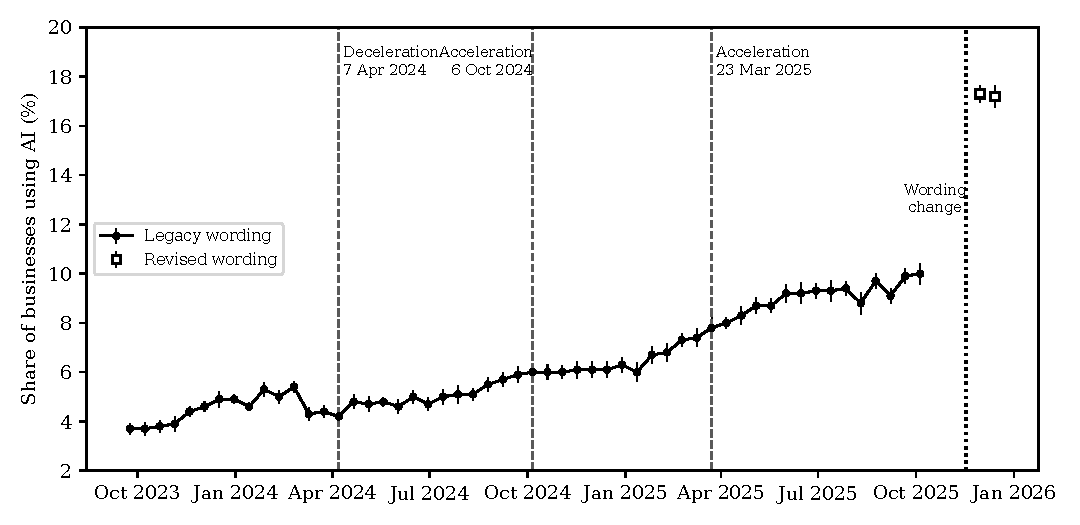
\includegraphics[width=\textwidth]{fig_series.pdf}
\caption{National estimate of the share of businesses using artificial intelligence, September 2023 to December 2025, with 95 percent intervals. Dashed vertical lines mark the two declarations. The dotted vertical line marks the wording change of 17 November 2025. Circles: legacy wording; open squares: revised wording.}
\label{fig:series}
\end{figure}

\begin{table}[t]
\small\centering
\caption{Epochs of the regime-aware monitor on the national series ($\tau = 0.01$, $\alpha = 0.05$). Curvature is the estimate $A_n/B_n$ at declaration with a 95 percent half-width, conditional on the published standard errors. Peak E is the value at declaration, or the maximum over the epoch when it ends without one; for the last epoch the anytime-valid p-value is 0.105.}
\label{tab:decl}
\begin{tabular}{lrllcr}
\toprule
Epoch start & Waves & Declaration & Date & Curvature (pp per wave$^2$) & E \\
\midrule
24 Sep 2023 & 15 & Deceleration & 7 Apr 2024 & $-0.0390 \pm 0.0262$ & 131.3 \\
21 Apr 2024 & 13 & Acceleration & 6 Oct 2024 & $0.0276 \pm 0.0196$ & 70.5 \\
20 Oct 2024 & 12 & Acceleration & 23 Mar 2025 & $0.0417 \pm 0.0302$ & 55.0 \\
6 Apr 2025 & 16 & None & --- & --- & 18.0 \\
\bottomrule
\end{tabular}

\end{table}

Figure \ref{fig:series} and Table \ref{tab:decl} give the results. The first epoch begins on 24 September 2023 and the deceleration monitor declares on 10 March 2024, after 13 waves, with an estimated curvature of $-0.028 \pm 0.010$ points per squared wave. The declaration is triggered by a single wave: the estimate falls from 5.4 to 4.3 percent, a change of $-6.2$ combined standard errors, the largest within-regime change in the series, and the e-value moves from 1.2 to $1.0 \times 10^5$ in that wave. The estimate stays near 4.4 afterwards. The cross-strata check finds three of the seven size classes beyond their own 95th percentile with the same sign at that wave, which is the only legacy wave with three or more, against seven of seven at the wording change. The evidence therefore does not distinguish a genuine fall in business use from an unannounced collection or processing change. If the wave is dropped, the first declaration is a deceleration on 24 March 2024 and the second is unchanged; if the wave is treated as the start of a new level that persists, there is no first declaration and the sequence becomes three decelerations (30 June 2024, 12 January 2025, 27 July 2025) with no acceleration. The first declaration should be read as conditional on the March 2024 wave being a feature of the population.

The second epoch begins on 24 March 2024 and the acceleration monitor declares on 6 April 2025, after 28 waves, with an estimated curvature of $0.0047 \pm 0.0017$: the growth rate was rising by about 0.1 points per wave over 20 waves. The third epoch begins on 20 April 2025 and runs through the wording change; the deceleration monitor, which responds to the flattening of the series through August 2025, peaks at 19.0 on 7 September 2025, an anytime-valid p-value of 0.105, and does not declare. The acceleration monitor stays below 1.1. The two revised-wording waves are retained with a level of their own.

\subsection{Sensitivity}
\label{sec:sensitivity}

\begin{table}[t]
\small\centering
\caption{Declarations with the published standard errors multiplied by the stated factor (1.55 is the robust estimate from the second differences).}
\label{tab:kappa}
\begin{tabular}{lccc}
\toprule
SE inflation & First declaration (E) & Second declaration (E) & Peak E, third epoch \\
\midrule
1.00 & 10 Mar 2024 ($1.0\times 10^{5}$) & 6 Apr 2025 ($1.9\times 10^{5}$) & 19.0 \\
1.25 & 10 Mar 2024 (834.9) & 6 Apr 2025 ($1.5\times 10^{3}$) & 5.3 \\
1.50 & 10 Mar 2024 (72.7) & 6 Apr 2025 (117.5) & 2.9 \\
1.55 & 10 Mar 2024 (52.0) & 6 Apr 2025 (81.8) & 2.7 \\
\bottomrule
\end{tabular}

\end{table}

The two declarations are stable to the prior scale: for $\tau$ from 0.005 to 0.04 they occur on the same two dates, and for $\tau = 0.0025$ the first is two weeks later (24 March 2024). They are stable in date to inflated standard errors up to the estimated factor of 1.55 (Table \ref{tab:kappa}), but not in strength: the e-values fall from about $10^5$ to 52 and 82, barely above the threshold. They are stable to a tolerance of $\gamma_0 = 0.001$ (e-values $4.5 \times 10^4$ and 917); with $\gamma_0 = 0.002$ the second moves to 20 April 2025 (e-value 194). The third epoch is not stable. With $\tau = 0.02$ the deceleration is declared on 7 September 2025 (E = 89) and with $\tau = 0.04$ on 10 August 2025 (E = 45); at $\alpha = 0.10$ it is declared on 10 August 2025; with standard errors inflated by 1.25 the peak falls to 5.3. Replacing the published standard errors by their median of 0.15 gives a different sequence (10 March 2024, 23 March 2025, 10 August 2025), so the outcome of the third epoch depends on the weights given to individual waves. The summer 2025 slowdown is best described as inconclusive.

\subsection{The wording change}
\label{sec:break}

\begin{table}[t]
\small\centering
\caption{Employment size classes at the wording change. Ratio is the first revised estimate over the last legacy estimate; jump is the standardized change; the 95th percentile is that of the class's standardized wave-to-wave changes within the legacy regime. The last column gives the date on which the pooled monitor declares an acceleration, where it does.}
\label{tab:strata}
\begin{tabular}{lccccc}
\toprule
Size class & Last legacy & First revised & Jump $|z|$ & 95th pct. within & Pooled declares at redesign \\
\midrule
1--4 & 11.0 & 17.0 & 13.2 & 2.77 & 30 Nov 2025 \\
5--9 & 8.6 & 15.5 & 8.7 & 2.85 & 30 Nov 2025 \\
10--19 & 8.1 & 17.8 & 10.6 & 2.37 & 30 Nov 2025 \\
20--49 & 7.0 & 18.7 & 13.8 & 1.96 & 30 Nov 2025 \\
50--99 & 9.7 & 20.7 & 9.7 & 2.29 & 30 Nov 2025 \\
100--249 & 8.8 & 23.7 & 8.6 & 1.74 & no \\
250+ & 13.0 & 30.5 & 6.1 & 2.31 & no \\
\bottomrule
\end{tabular}

\end{table}

Between the last legacy wave (10.0 percent, 5 October 2025) and the first revised wave (17.3 percent, 30 November 2025) the estimate rose by 7.3 points, which is 25.7 combined standard errors, against a within-regime median absolute standardized change of 0.94 and a maximum of 6.2. The regime-aware monitor books no evidence from it, by construction, and with two waves in the new regime this says little beyond that the transition wave is absorbed. The pooled analysis declares an acceleration on 30 November 2025 with an E-value of order $10^{123}$, and a repeated curvature test applied to the spliced series has a statistic of 36.4 in magnitude at that wave.

Table \ref{tab:strata} shows that all seven size classes jump in the same wave and in the same direction, by 6.1 to 13.8 standard errors and by 2.6 to 7.0 times their own 95th percentile (1.74 to 2.85). The ratio of the first revised to the last legacy estimate, 1.55 to 2.69, rises with the level of the class, so the effect on the scale of the series is closer to proportional than to a constant; at the national level the ratio is 1.73. With two revised waves we cannot test whether the effect is additive, and Table \ref{tab:redesign} shows that this matters once the new regime is longer.

\subsection{Comparison with repeated testing}
\label{sec:comparison}

The curvature $z$ statistic was applied at each wave to the series with the same restart rule, with regime columns and without. The uncorrected test declares nine times, the first on 19 November 2023. The Bonferroni rule, using the remaining length of the series as its horizon, declares on 10 March 2024, 6 April 2025, 10 August 2025 and 21 September 2025; the last two are the summer 2025 slowdown, which the e-process at $\tau = 0.01$ does not declare, as expected from the loss of power in Table \ref{tab:power}. The spending rule declares six times, with the first and the last two on the same dates as the Bonferroni rule. A moving-average rule, which crosses when the sign of the 3-wave mean minus the 8-wave mean changes, crosses four times (24 March 2024, 19 May 2024, 7 September 2025, 21 September 2025). Without regime columns the Bonferroni and spending rules add a declaration on 14 December 2025 and the uncorrected rule declares on 30 November 2025, at the revised-wording waves. With regime columns the first two dates agree with the e-process. The e-process is therefore not distinguished on the real data by what it finds; its advantage is the guarantee, at a cost in power.

\subsection{Extensions applied to the BTOS series}
\label{sec:extapp}

\begin{table}[t]
\small\centering
\caption{Declarations of the monitor variants on the national series. The prior scale is 0.01 except where stated. Dec.: deceleration; acc.: acceleration.}
\label{tab:extapp}
\begin{tabular}{lp{9.5cm}}
\toprule
Monitor & Declarations \\
\midrule
Known scale, single $\tau$ & 10 Mar 2024 (dec.); 6 Apr 2025 (acc.) \\
Unknown scale & 7 Apr 2024 (dec.); 6 Oct 2024 (acc.); 6 Apr 2025 (acc.) \\
Mixture over $\tau$ & 10 Mar 2024 (dec.); 6 Apr 2025 (acc.); 7 Sep 2025 (dec.) \\
Regime slopes and guard waves & 10 Mar 2024 (dec.); 6 Apr 2025 (acc.) \\
Log scale, $\tau = 0.002$ & 10 Mar 2024 (dec.); 4 May 2025 (acc.) \\
\bottomrule
\end{tabular}

\end{table}

\begin{table}[t]
\small\centering
\caption{Smoothed slope (percentage points per wave, with 95 percent half-width) of a local linear trend model with the published standard errors multiplied by a common factor, and a level intervention at the wording change. The maximum-likelihood estimate of the factor is 1.65.}
\label{tab:ssm}
\begin{tabular}{lcc}
\toprule
Date & Slope, scale estimated & Slope, published SE \\
\midrule
10 Mar 2024 & $-0.12 \pm 0.11$ & $-0.24 \pm 0.16$ \\
30 Jun 2024 & $0.10 \pm 0.11$ & $0.09 \pm 0.17$ \\
17 Nov 2024 & $0.05 \pm 0.12$ & $0.03 \pm 0.18$ \\
6 Apr 2025 & $0.28 \pm 0.12$ & $0.29 \pm 0.18$ \\
27 Jul 2025 & $0.05 \pm 0.12$ & $-0.02 \pm 0.18$ \\
5 Oct 2025 & $0.12 \pm 0.25$ & $0.20 \pm 0.39$ \\
\bottomrule
\end{tabular}

\end{table}

Table \ref{tab:extapp} gives the declarations of the variants. The unknown-scale monitor, which estimates the scale of the errors within each epoch, declares a deceleration on 7 April 2024 (E = 206), four weeks after the known-scale monitor, then an acceleration on 6 October 2024 (E = 43, barely above the threshold) and the acceleration on 6 April 2025 (E = 64); its last epoch, which starts on 20 April 2025, peaks at 3.6, so the summer 2025 slowdown is not evidence for it. It is the version whose guarantee does not rely on the published standard errors, and it supports the acceleration of spring 2025 and a deceleration in early 2024, and little else. The mixture over the prior scale declares the same two dates as the single scale and, in addition, the summer 2025 deceleration on 7 September 2025 (E = 51). The two readings are consistent with Subsection \ref{sec:sensitivity}: the slowdown is declared when the published standard errors are taken at face value and a prior scale that is not too narrow is allowed, and it is not when the scale is estimated. Regime slopes and guard waves change nothing before the wording change, because the two revised waves are absorbed. On the log scale the first declaration is unchanged and the acceleration moves to 20 April 2025 or 4 May 2025, depending on the prior scale in log units (0.001 or 0.002 to 0.004).

A local linear trend model, which is what a user of structural time series would fit, estimates the slope and its change directly. Its maximum-likelihood estimate of the scale factor on the published standard errors is 1.65, in line with the second-difference estimate of 1.55 and with the dispersion in Subsection \ref{sec:dispersion}. Table \ref{tab:ssm} shows the smoothed slope. Around March 2024 it is negative ($-0.12 \pm 0.11$ points per wave), through 2024 it is between 0.05 and 0.10, in April 2025 it is $0.28 \pm 0.12$, in July 2025 it is $0.05 \pm 0.12$, whose interval excludes the April value, and in October 2025 it is $0.12 \pm 0.25$. This says more than the declarations about how large the changes were and how uncertain: the acceleration in April 2025 and the slowdown of the summer are of the size of 0.2 points per wave, with intervals of $\pm 0.12$. The standardized one-step innovations of the same model with the scale estimated have a standard deviation of 1.05 and autocorrelations of $-0.06$, $0.21$ and $-0.43$ at lags 1, 2 and 3 and $0.14$ and $-0.10$ at lags 6 and 12, from 46 waves, against a band of about $\pm 0.29$. There is no evidence of dependence at the lag at which a panel returns, and there is some at lag 3, which we attribute to the single large drop in March 2024 and have not investigated further.

\section{Discussion}
\label{sec:discussion}

\subsection{Implications for agencies and users}
\label{sec:implications}

Agencies that announce a redesign should publish the regime label with the series, and, for a redesign whose effect is unlikely to be additive, a parallel run or a bridge; the monitor needs the label, and with the guard an error of one wave costs 14 percent of the information. Users who monitor a series should report the epoch, the estimated curvature and its standard error, and the sensitivity to the standard errors, in addition to the e-value. The unknown-scale version is the one to use when the standard errors are not trusted, which the BTOS dispersion suggests they should not be. The e-process is a complement to a state-space model with an intervention, which estimates the slope and its change directly and was more informative about size in the application; it is useful where a user wants a stopping rule with a stated error probability that holds however often the series is inspected.

\subsection{Limitations}
\label{sec:limitations}

The extensions remove the assumptions of known scale, additive redesign effects, exact regime dates and a fixed prior scale, but not all assumptions. The unknown scale is a common factor: standard errors that are wrong by wave-specific amounts, which the published ones may be, since the national ones range from 0.08 to 0.23 points, are not covered, and the proof still takes the weights as fixed. Positive dependence between waves one panel cycle apart is covered only by simulation and by a diagnostic that finds no evidence in 46 innovations. The unknown-scale version does not include the tolerance for small curvature, and the proportional-effect version leaves almost no information after a redesign. The null is a statement about shape, and a declaration says that the path has curved, not why; the first declaration in the application is driven by one large drop that may be a measurement event, and the cross-strata check is a screening rule. Declarations depend on where the epoch starts, and the dates are crossing times. The data are an archived final series ending in December 2025, the post-redesign run is two waves long, and nonresponse bias that drifts over time is absorbed into the latent path.

\section{Conclusion}
\label{sec:conclusion}

A published survey series can be monitored for changes in its growth rate with error control that holds under continuous inspection, for any unknown level and slope and for redesign shifts at announced dates. The basic monitor needs the published standard errors to be right, the shifts to be additive and the dates to be exact; the extensions remove each of these in turn, at a cost in information that we quantify. Applied to the BTOS series on business use of artificial intelligence, all versions find an acceleration in spring 2025 and a deceleration in early 2024 that is triggered by one large drop; the summer 2025 slowdown is declared when the published standard errors are taken at face value and not when their scale is estimated, and a state-space model puts its size at about 0.2 points per wave with an interval of $\pm 0.12$.

\appendix

\section{Proof of Proposition \ref{prop:valid} and Corollary \ref{cor:epochs}}
\label{app:proof}

Fix an epoch and write $\mathcal{X}_n = \mathrm{span}(D_n) \subset \mathbb{R}^n$. Under model \eqref{eq:model} the vector $y_{1:n}$ equals $D_n c + \gamma q_{1:n} + e_{1:n}$ for some $c \in \mathbb{R}^p$ and $e_{1:n} \sim \mathcal{N}(0, W_n^{-1})$. Let $G_n$ be the $\sigma$-field generated by $R_n = M_n y_{1:n}$, that is, by $y_{1:n}$ modulo $\mathcal{X}_n$. The columns of $D_{n+1}$ restricted to the first $n$ rows span $\mathcal{X}_n$, with a new regime column being zero on earlier rows, so $y_{1:n} + \mathcal{X}_n$ is a function of $y_{1:n+1} + \mathcal{X}_{n+1}$ and $(G_n)$ is a filtration. Moreover $B_{n+1} \ge B_n$: the residual of $q$ on the larger design restricted to the first $n$ rows is no larger in the $W$-norm than the residual on $D_n$, and the new row adds a nonnegative term.

In the inner product $\langle u, v \rangle_W = u^\top W_n v$, $M_n$ is the orthogonal projector onto $\mathcal{X}_n^{\perp}$. The vector $R_n$ is a standard Gaussian on $\mathcal{X}_n^{\perp}$ with mean $\gamma M_n q$, and its law does not depend on $c$. Write $u = \delta - \gamma_0$ for a candidate curvature $\delta > \gamma_0$ and $A_n^{+} = A_n - \gamma_0 B_n$, where $\langle M_n q, R_n \rangle_W = A_n$ and $\langle M_n q, M_n q\rangle_W = B_n$. The density ratio of $R_n$ under curvature $\delta$ against curvature $\gamma_0$ is
\[
L_n(u) = \exp\!\big(u A_n^{+} - \tfrac{1}{2} u^2 B_n\big).
\]
For $\gamma = \gamma_0$, $(L_n)$ is the likelihood ratio of the observation $R_n$ of fixed law on the increasing sequence $G_n$ and is a nonnegative martingale with initial value one. Mixing over $u > 0$ with the half-normal law keeps this and gives $E_n^{+}$ by evaluating the Gaussian integral,
\[
\int_0^\infty e^{u A - u^2 B/2}\, \frac{2}{\tau\sqrt{2\pi}} e^{-u^2/(2\tau^2)}\, du
= \frac{2}{\tau\sqrt{a}}\, \Phi\!\Big(\frac{A}{\sqrt{a}}\Big) e^{A^2/(2a)}, \qquad a = B + \tau^{-2}.
\]
For $\gamma < \gamma_0$, conditionally on $G_{n-1}$ the increment $A_n^{+} - A_{n-1}^{+}$ is normal with mean $(\gamma - \gamma_0)(B_n - B_{n-1})$ and variance $B_n - B_{n-1}$ (the innovation of a Gaussian regression in sequentially orthogonalized form). Hence $\E[L_n/L_{n-1} \mid G_{n-1}] = \exp(u(\gamma - \gamma_0)(B_n - B_{n-1})) \le 1$ for $u > 0$, because $B_n - B_{n-1} \ge 0$, and the mixture is a supermartingale. Ville's inequality gives $\Prob(\sup_n E_n^{+} \ge 2/\alpha) \le \alpha/2$ for all $c$. The case of $E^{-}$ is the same with the sign of $A_n$ reversed. This proves Proposition \ref{prop:valid}.

For Corollary \ref{cor:epochs}, condition on the history up to the stopping time at which the epoch starts. Given the history, the future waves obey the model and the latent path is a fixed function. If the path is linear on the first $n^{*}$ waves of the epoch, a declaration at $n \le n^{*}$ is an event of the type bounded in Proposition \ref{prop:valid}, applied to the model whose path is the linear extension, which has the same law of the data up to $n^{*}$. If the path is linear throughout, each epoch ends in a declaration with conditional probability at most $\alpha$, so $\Prob(N \ge m) \le \alpha^m$ and $\E[N] = \sum_{m \ge 1} \Prob(N \ge m) \le \alpha/(1-\alpha)$.

For Proposition \ref{prop:scale}, let $\mathcal{X}_n$ be as above and write $R_n = M_n y_{1:n}$. Under $\gamma = 0$ the law of $R_n$ is $\mathcal{N}(0, \kappa^2 I)$ on $\mathcal{X}_n^{\perp}$ in the $W$-geometry, for every $c$. The group of location shifts in $\mathcal{X}_n$ and positive scalings acts on the data; a maximal invariant is the direction $u_n = R_n/\|R_n\|$, whose law under $\gamma = 0$ is uniform on the sphere of dimension $\nu_n$ for every $c$ and $\kappa$. Under curvature $\gamma$ the vector $R_n$ is $\mathcal{N}(\gamma m_n, \kappa^2 I)$ with $m_n = M_n q$ and $\|m_n\|^2 = B_n$, and the density of $u_n$ depends on $(\gamma, \kappa)$ only through $\delta = \gamma/\kappa$. In polar coordinates $R_n = \rho u_n$ the density of $u_n$ relative to the uniform law is proportional to $e^{-\delta^2 B_n/2}\int_0^\infty \rho^{\nu_n - 1} e^{-\rho^2/2 + \rho \delta \langle u_n, m_n\rangle}\, d\rho$, with $\langle u_n, m_n \rangle = A_n/\sqrt{\mathrm{RSS}_n} = s_n$, which is $L_n(\delta)$ in \eqref{eq:unknown}. The $\sigma$-fields of $u_n$ are nested: $R_n$ is a linear function of $R_{n+1}$, and hence $u_n$ is a function of $u_{n+1}$ whenever $R_n \ne 0$, which holds almost surely. So $L_n(\delta)$ is a likelihood ratio of increasing observations of fixed null law, a nonnegative martingale with mean one, and so is its mixture $E_n^{\sigma,+}$; Ville's inequality gives the bound. The monitor for deceleration is the same with $\delta < 0$. We checked the unit mean numerically: at $n = 12$ the mean of $E_n^{\sigma,+}$ over 4,000 simulated null paths was 1.001 for $\kappa = 1$ and 1.018 for $\kappa = 2$.

Regime slopes and guard waves enlarge $D_n$ by columns that, like the regime levels, are zero on rows before the regime begins (for regime slopes) or are unit vectors on single rows (for guard waves), so the nesting argument and Proposition \ref{prop:valid} apply unchanged.

\section{Computation}
\label{app:computation}

For each epoch, at each wave $n$ with $B_n > 0$ the weighted regression of $y$ and $q$ on regime indicators and $t$ gives the residuals; $A_n$ and $B_n$ follow from \eqref{eq:AB}, and $E_n^{\pm}$ is evaluated on the logarithmic scale. If $\max(E_n^{+}, E_n^{-}) \ge 40$ a declaration is recorded and the next epoch starts at wave $n+1$. The unknown-scale e-value is computed by quadrature over $\delta$ on a grid of 24 prior quantiles and 29 points around the maximum of the integrand, with the radial integral evaluated on a grid around its mode, all on the logarithmic scale. All results were produced by the scripts in the replication package, from the data of Subsection \ref{sec:data}.

\section*{Declaration of Conflicting Interests}
The Author declares that there is no conflict of interest.

\section*{Funding}
The Author received no financial support for the research, authorship, and/or publication of this article.

\section*{Data Availability}
All data are public statistics of the U.S. Census Bureau (Business Trends and Outlook Survey, \url{https://www.census.gov/hfp/btos/data_downloads}). The analysis data set and the code that reproduces every number, table and figure are provided with the submission.

\bibliographystyle{chicago}
\bibliography{refs}

\end{document}
